\documentclass[ngerman,aspectratio=169,10pt]{beamer}

\usetheme[progressbar=frametitle]{metropolis}
\usepackage{appendixnumberbeamer}

\graphicspath{{./graphics/}}

\usepackage{booktabs}
\usepackage{xspace}
\usepackage{amsmath}
\usepackage{amssymb}
\usepackage{amsthm}
\usepackage{xfrac}
\usepackage{verbatim}

\usepackage{stmaryrd}

\title{KCT als Multi-Commodity-Flow-Formulierung (MCF)}
% \subtitle{}
% \date{16. November 2020}
\author{Finn Stutzenstein, Levin Nemesch, Joshua Sangmeister}
\institute{Algorithm Engineering - Übung 4}
\titlegraphic{
    \hfill
\includegraphics[height=1.5cm]{unilogo.pdf}\\[-0.2cm]
    \hspace*{8.3cm} \textsc{AG Theoretische Informatik}
}

\begin{document}
	
\maketitle

\begin{frame}{Definitionen}
    \begin{itemize}
        \item $V' := V \cup \{r\}$
        \item $A := \{(v, w), (w, v) \mid \{v, w\} \in E\}$
        \item $A_r := \{(r, v) \mid v \in V\}$
        \item $A' := A \cup A_r$
        \item gerichteter Graph $G'=(V', A')$
        \item Nachbarknoten von v: $N(v) := \{w \in V'  \mid \{v, w\} \in E'\}$
        \item Flussvariable $f^u_{(v,w)}$ modelliert Fluss der Stärke $y_u$ von $r$ nach $u$ über die Kante $(v,w)$
    \end{itemize}
\end{frame}

\begin{frame}{MCF ILP}
	\begin{align*}
    	\min && c^Tz & &&\\
    	\text{s.t.} && z(A) &= k &&\\
    	&& y(V) &= k+1 &&\\
    	&& z(A_r) &= 1 &&\\
    	&& \sum_{w\in N(v)} f^u_{(w,v)} - \sum_{w\in N(v)} f^u_{(v,w)} &= \begin{cases}
    	        y_u & v=u\\
    	        0 & \text{sonst}
    	\end{cases} &\forall& u, v\in V\\
    	&& 0 \leq f^u_{(v,w)} &\leq z_{(v,w)} &\forall& (v, w) \in A', u \in V\\
    	&& z_a, y_v &\in \{0, 1\} &\forall& a \in A, v \in V
	\end{align*}
\end{frame}

\begin{frame}{Eigenschaften von MCF}
    \begin{itemize}
        \item Analog zu DCut:
        \begin{itemize}
            \item Extra Knoten $r$
            \item Zusätzliche Kanten $\{r\}\times V$
            \item Flüsse sind gerichtet
            \item Wählt nur eine der Kanten von $r$
        \end{itemize}
        \item Wählt $k$ Kanten aus $A$ und $k+1$ Knoten aus $V$ $\Rightarrow$ Keine Kreise möglich
        \item Flussbedingungen stellen Graphzusammenhang her.
    \end{itemize}
\end{frame}

\begin{frame}{Flussbedingungen}
    \begin{itemize}
        \item Existiert ein Fluss an einer Kante, muss die Kante gewählt werden
        \item Sei $v$ gewählt ($y_v=1$), dann existiert ein Pfad von $r$ nach $v$ mit dem Fluss 1. Flussbedingung für $v$:
        \[\sum_{w\in N(v)} f^v_{(w,v)} - \sum_{w\in N(v)} f^v_{(v,w)}=1\]
        \[\Rightarrow\exists w\in N(v):f^v_{(w,v)}=1\]
        \[\Rightarrow \sum_{x\in N(w)} f^v_{(x,w)} - \sum_{x\in N(w)} f^v_{(w,x)}=0\]
        \[\Rightarrow \exists x\in N(w):f^v_{(x,w)}=1\text{~... bis~}r\]
        \item Sei $(r,a)$ die von $r$ gewählte Kante. Dann führen alle Pfade über $a$.\\
        Folgerung: Der Graph ist zusammenhängend.
    \end{itemize}
\end{frame}

\begin{frame}{MCF echt stärker als UCut: $\exists$-Teil}
    \centering
    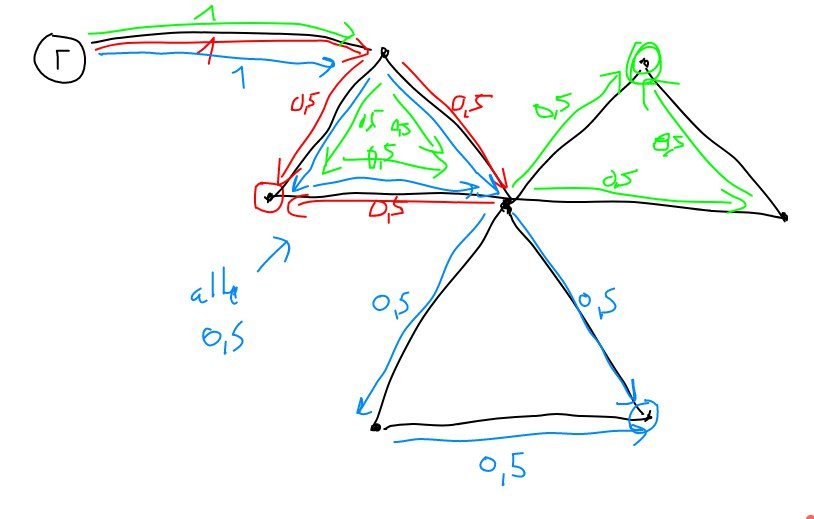
\includegraphics[width=300px]{invalid.jpg}
\end{frame}

\begin{frame}{MCF echt stärker als UCut: $\forall$-Teil}
    Projektion einer zulässigen MCF Lösung $(z'_{(v,w)}, y'_v,f'^u_{(v,w)})$ auf eine UCut Lösung $(x'_e, y'_v)$:
    \[x_{\{v,w\}}=z'_{(v,w)}+z'_{(w,v)}\]
    (Lasse $f'$ fallen) Ist UCut Lösung zulässig?
    \begin{itemize}
        \item 0/1-Schranken: $y'_v$ passt, $x'_e$: O.B.d.A. gilt $z_{(u,v)}+z_{(v,u)}\leq1$. Passt
        \item $\pmb{x}(E)$, $\pmb{y}(V)$: Analoge Constraints. Passt
        \item $\pmb{x}(\delta(W))\geq y_v+y_w-1$:\\
        Angenommen es existiert $W$, sodass $v$ und $w$ gewählt sind und $\pmb{x}(\delta(W))<1$.\\
        Da beide Knoten gewählt sind existiert ein (ungerichteter) Fluss von $v$ über $r$ nach $w$ mit einer Kapazität von 1. Nach dem max-flow-min-cut Theorem muss ein Schnitt mit mindestens 1 existieren. \hfill\mbox{\Large{$\lightning$}}
    \end{itemize}
\end{frame}

\begin{frame}{MCF vs. DCut}
\begin{tabular}{c|c|c}\hline
   & DCut  & MCF \\\hline
Praktische Größe Zfkt: & $2|E|$ & $2|E|$ \\\hline
Anzahl Constraints & $1+1+|V|+|V|\cdot2^{|V|-1}$ & $1+1+1+|V|^2+|V|(2|E|+|V|)$ \\\hline
Anzahl binäre Variablen & $|V|+2|E|$ & $2|V|+2|E|$ \\\hline
Anzahl reelle Variablen & $0$ & $|V|(2|E|+|V|)$\\\hline
\end{tabular}
\end{frame}

\begin{frame}{MCF vs. DCut}
\begin{quote}
The MCF formulation requires only a polynomial number of variables and constraints. However, the sheer number of variables becomes a practical drawback of this approach. In addition to the $x$ and $y$ variables, we require $|V|\cdot|A|$ variables to model the flow. As we know from similar problems [...], this leads to poor performance of MCFs in practice, compared to directed cut-based approaches, which allow efficient separation of their exponentially many constraints.
\end{quote}
\begin{flushright}
--- M. Chimani et al: Obtaining optimal k-cardinality trees fast. \textit{ACM Journal of Experimental Algorithmics}, 14 (2009)
\end{flushright}
\end{frame}
\end{document}